\chapter{Results}
\section{Babel Stream}\label{sec:res-babel}
Babel Stream's results show that Rust and Rayon are unable to scale as well as C++ and OpenMP\@. Figures~\ref{fig:babel-dot},~\ref{fig:babel-add} and~\ref{fig:babel-triad} all show that Rust and C++ have similar performance but that at higher thread counts, there is a great deal of difference between the threading performance of both implementations. In each figure, 1gb refers to the size of the single array in that execution run, and chunk\_xxMB refers to how large a subsection of that array the threads are assigned to.

For example, both Rust and C++ having very similar memory bandwidths in the Dot product's serial execution, with Rust at 11.5 GB/s and C++ at 11.6 GB/s, giving a difference in bandwidth of just 1\%.
However, this difference later widens at 32 threads to 35\% with Rust at 87.3 GB/s and C++ at 135.1 GB/s.

\begin{figure}[h]
\centering
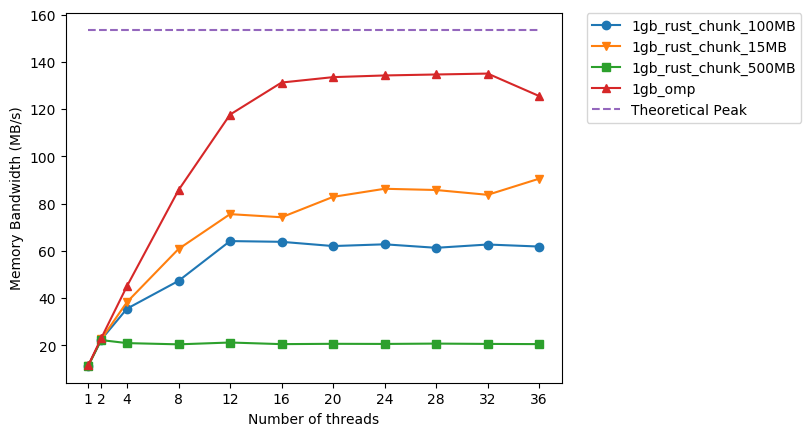
\includegraphics[width=.9\linewidth]{figs/babel/Dot.png}
\caption{Babel Stream --- Dot product bandwidth}\label{fig:babel-dot}
\end{figure}

Whilst the performance difference is not so pronounced for both the add and triad benchmarks, shown in Figure~\ref{fig:babel-add} and~\ref{fig:babel-triad} it is still quite prominent, with a performance difference of \% for add and \%\todo{numbers pls} for triad. It is interesting that the dot product is able to attain such a higher level of memory bandwidth. A deep investigation into why the dot product attains a higher bandwidth than the add or triad benchmarks was not completed. However, I believe the difference is likely due to the hardware's implementation of combined operational units, like fused multiply adds, as a cursory inspection of the assembly code here did not reveal any sufficient optimisations at that level.

It is noteworthy that the rate of improvement in memory bandwidth decreases sharpely between 16 and 20 threads. This decrease is probably due to each core only having 18 processors. Requiring data to passed across the CC-NUMA regions adds a signficant communication overhead, which slows the rate of increase in memory bandwidth.
\begin{figure}[h]
\centering
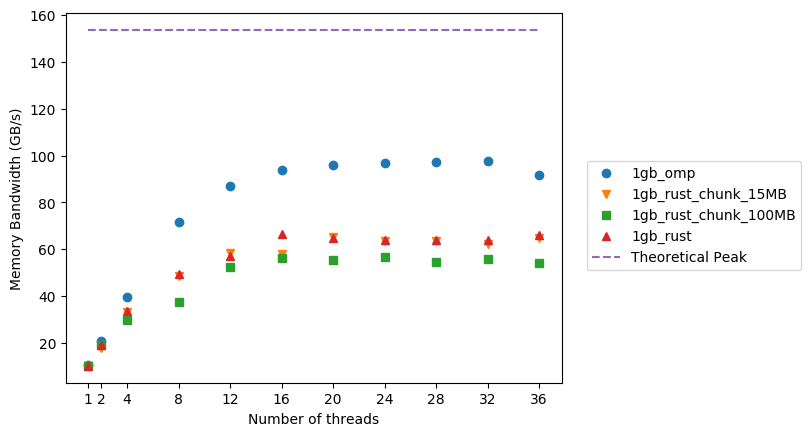
\includegraphics[width=.9\linewidth]{figs/babel/Add.png}
\caption{Babel Stream --- Add bandwidth}\label{fig:babel-add}
\end{figure}

This increasing difference lead me to believe that an examination of assembly code would not be beneficial in this circumstance, as it seemed like the low level, assembly implementation of both of the dot product was not that different. Instead, it seemed like the threading implementation was so different that it was what was causing the problem, which is much easier to understand in its high level expression. I decided to investigate the thread scheduling implementation.

\begin{figure}[h]
\centering
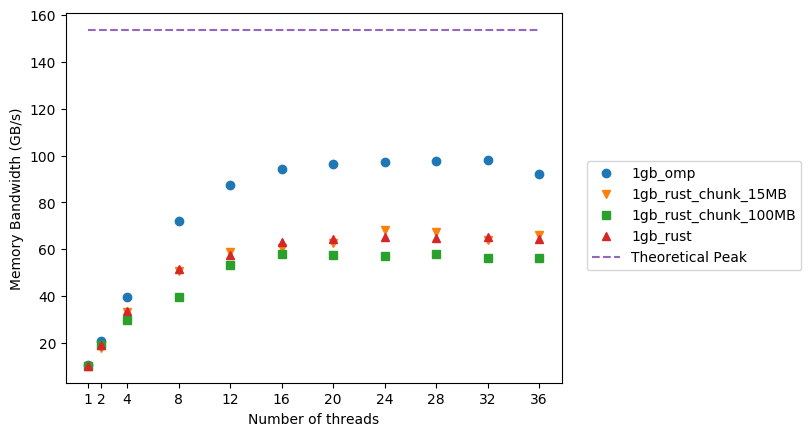
\includegraphics[width=.9\linewidth]{figs/babel/Triad.png}
\caption{Babel Stream --- Triad bandwidth}\label{fig:babel-triad}
\end{figure}

The decision to investigate thread scheduling was made because it was easy to investigate. There was also the possibility that Rayon's context switching was more costly to performance than OpenMP's. However, this would likely need to be confirmed at the level of assembly instructions, which can be difficult to parse, especially if you don't know what exactly you're looking for. Therefore, it seemed like a much better strategy to look at how thread scheduling in Rayon works  and also look out for hints of context switching costs.

Consulting the documentation reveals that Rayon's \texttt{par\_iter()} construct reveals that the parallel iterator API is a wrapper around Rayon's \texttt{join()} method~\cite{smallCult}. In the source code for \texttt{join()}, it is stated that the underlying implementation of join in Rayon is different to the common conception of it. 
`The underlying technique is called ``work stealing'': the
Rayon runtime uses a fixed pool of worker threads and attempts to only execute code in parallel when there are idle CPUs to handle it'~\cite{joinSrc}.

Work stealing is an established parallel technique, in which threads work on chunks of computation, and when they have finished their chunk, they steal chunks of computation from other threads~\cite{blumofe1999}. This reactive method of scheduling is very good at dealing with unaticipated work loads, when it is not known where the bulk of the computation will take place.

Unfortunately, a dynamic schedule will always do poorly when the workload is evenly distributed amongst threads, especially compared to static schedules. The defualt OpenMP parallalel for schedule is a static one, which evenly splits the work between threads~\cite{OpenMPSpec5}. The effect of this schedule is that data is more likely to work on data which it has initilised, which is likely to be within the same CC-NUMA region, and therefore quicker to access. In comparison, the work which threads will do in a work stealing schedule is non deterministic, and may require to be fetched from further away, at greater cost.

Although the results for Babel Stream do show that in this particular circumstance, OpenMP does have high performance, it does not necessarily follow that the static schedule will always be best for HPC. To investigate this further, I will now examine the SpMV results.
\section{Sparse Matrix Vector Multiplicationmatplotlib scatter }\label{sec:res-sparse}
\section{K-means clustering}
\section{Questionnaire}
Figure~\ref{fig:questions} presents the collected data from the questionnaire. Each small dot represents one answer, and a larger dot represents two. Eleven responses were collected in total.
These results show zero correlation between competency and score. This suggests that it is difficult to predict how easy a HPC programmer will understand Rust. 

\begin{figure}[h]
\centering
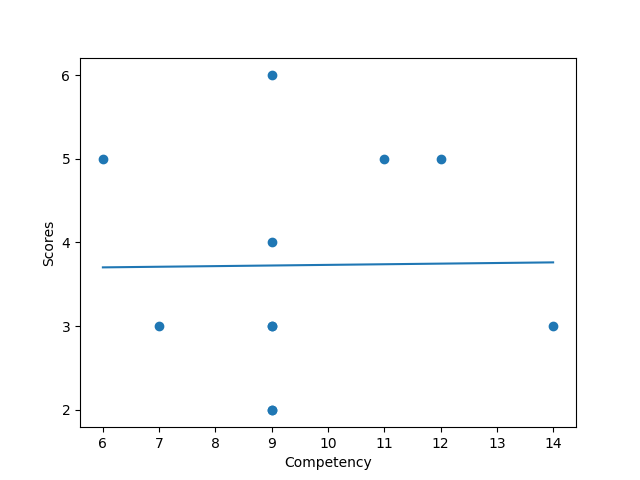
\includegraphics[width=.8\linewidth]{figs/questions/scatter.png}
\caption{Questionnaire --- Score against Competency}\label{fig:questions}
\end{figure}

However, as these such little data was collected in this circumstance, it would be unreasonable to claim that this study contains any decisive information. The study would need to be carried out a second time, with a much larger group of participants.

Interesting highlights from the data 
\todo{include data? Didn't say I would}
